% ===============================================================================================
% ===============================================================================================
% COMPUTER ARCHITECTURE REMINDER
%
% - Von neumann architecture
% - Memory model
% - memory pyramid
%
% ===============================================================================================
% ===============================================================================================
\subsection{Computer architecture reminder}


\begin{frame}[containsverbatim]
\frametitle{Von Neumann architecture}
\begin{center}
        {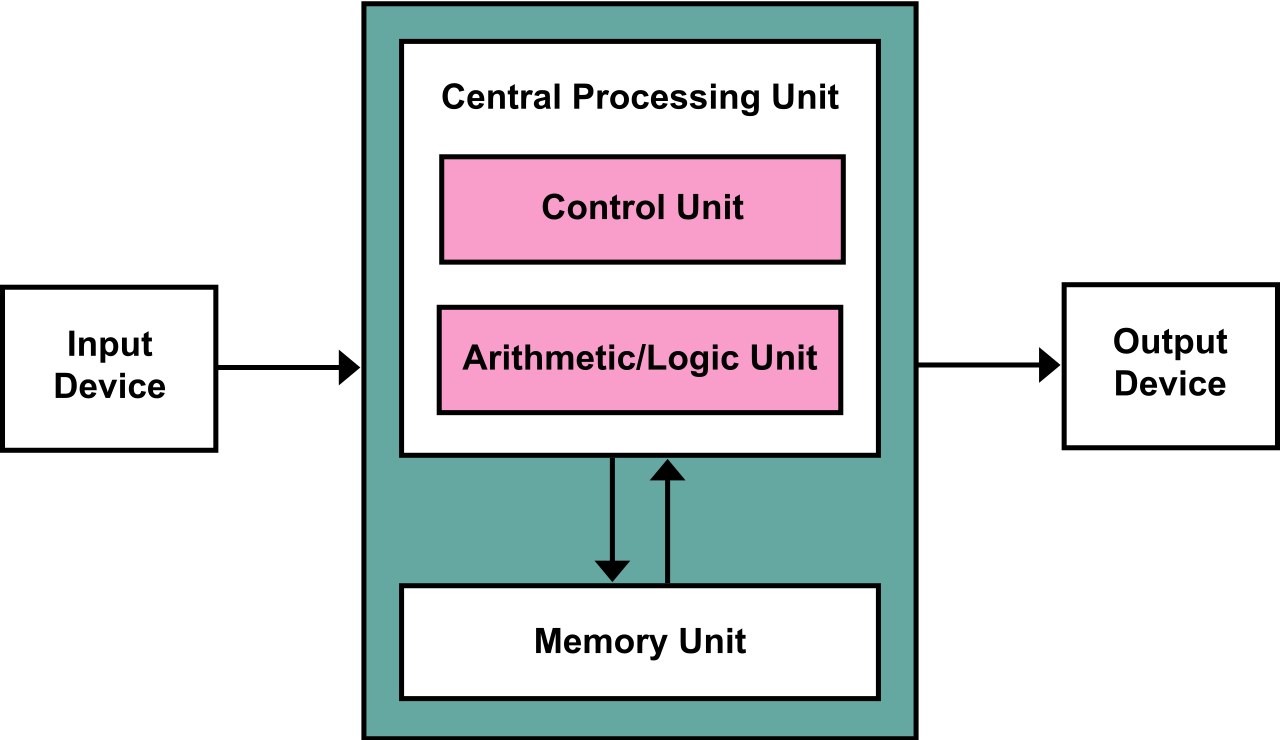
\includegraphics[height=3.5cm]{Day0/images/vonneumann.png}}
\end{center}
\begin{enumerate}
	\item{\textbf{ALU} Arithmetical and Logical Unit}
	\item{\textbf{Control Unit}}
	\item{\textbf{Memory}}
	\item{\textbf{Input/Output}}
\end{enumerate}
\end{frame}

\begin{frame}[containsverbatim]
\frametitle{System bus}
\begin{center}
        {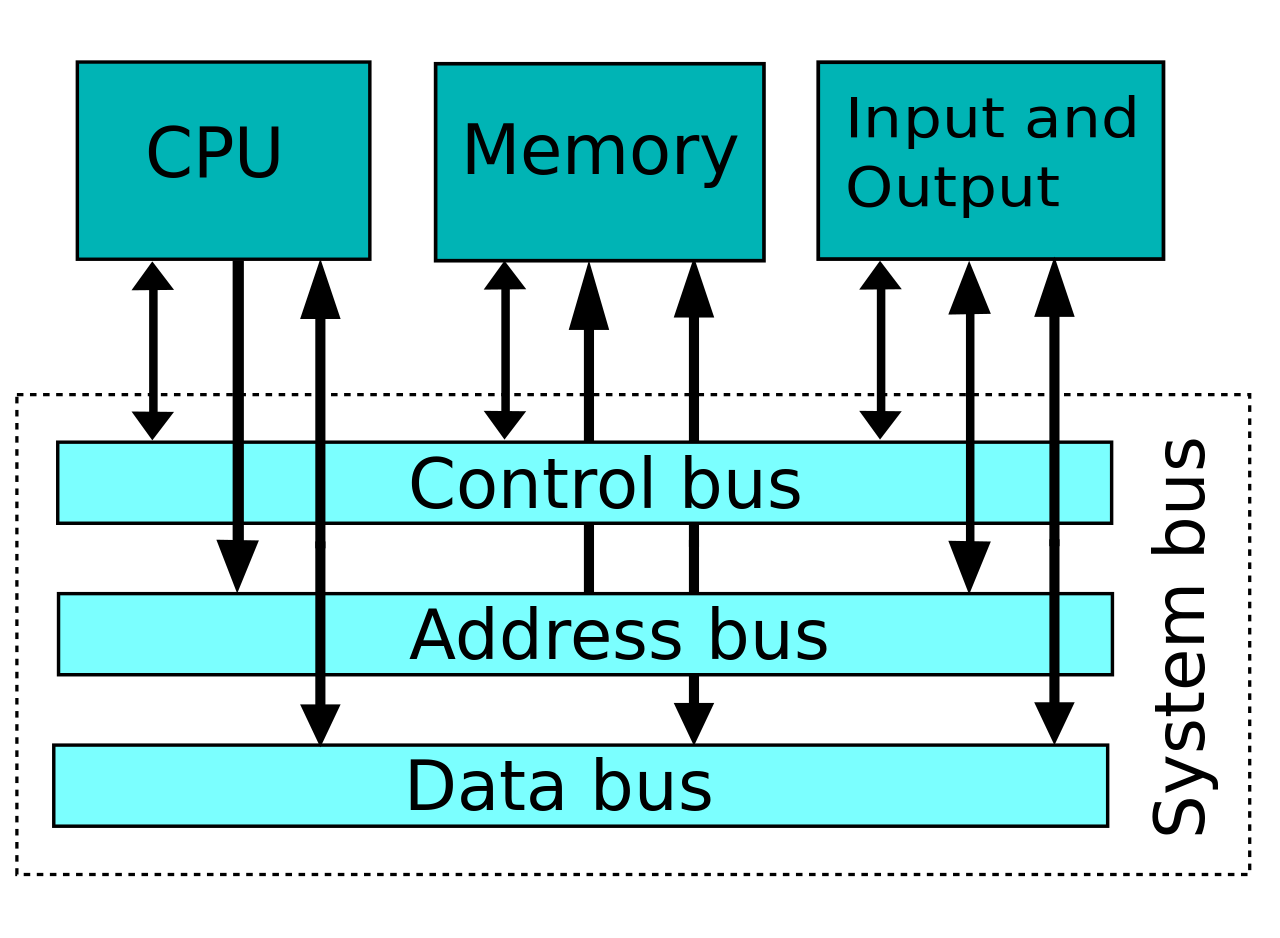
\includegraphics[height=4.5cm]{Day0/images/system-bus.png}}
\end{center}
\begin{itemize}
	\item{Address bus : instructions on \textit{where to find} the data}
	\item{Data bus : instructions on \textit{what to find}}
	\item{Control bus : instructions on \textit{what to do with} (for example : \texttt{read}, \texttt{write}, \texttt{fetch}, etc..}
\end{itemize}
\end{frame}

\begin{frame}[containsverbatim]
\frametitle{Memory pyramid}
\begin{center}
        {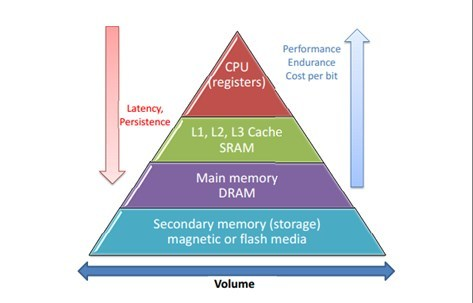
\includegraphics[height=5cm]{Day0/images/pyramid.png}}
\end{center}
\end{frame}

\begin{frame}[containsverbatim]
\frametitle{How does it look like in reality ?}
\begin{center}
        {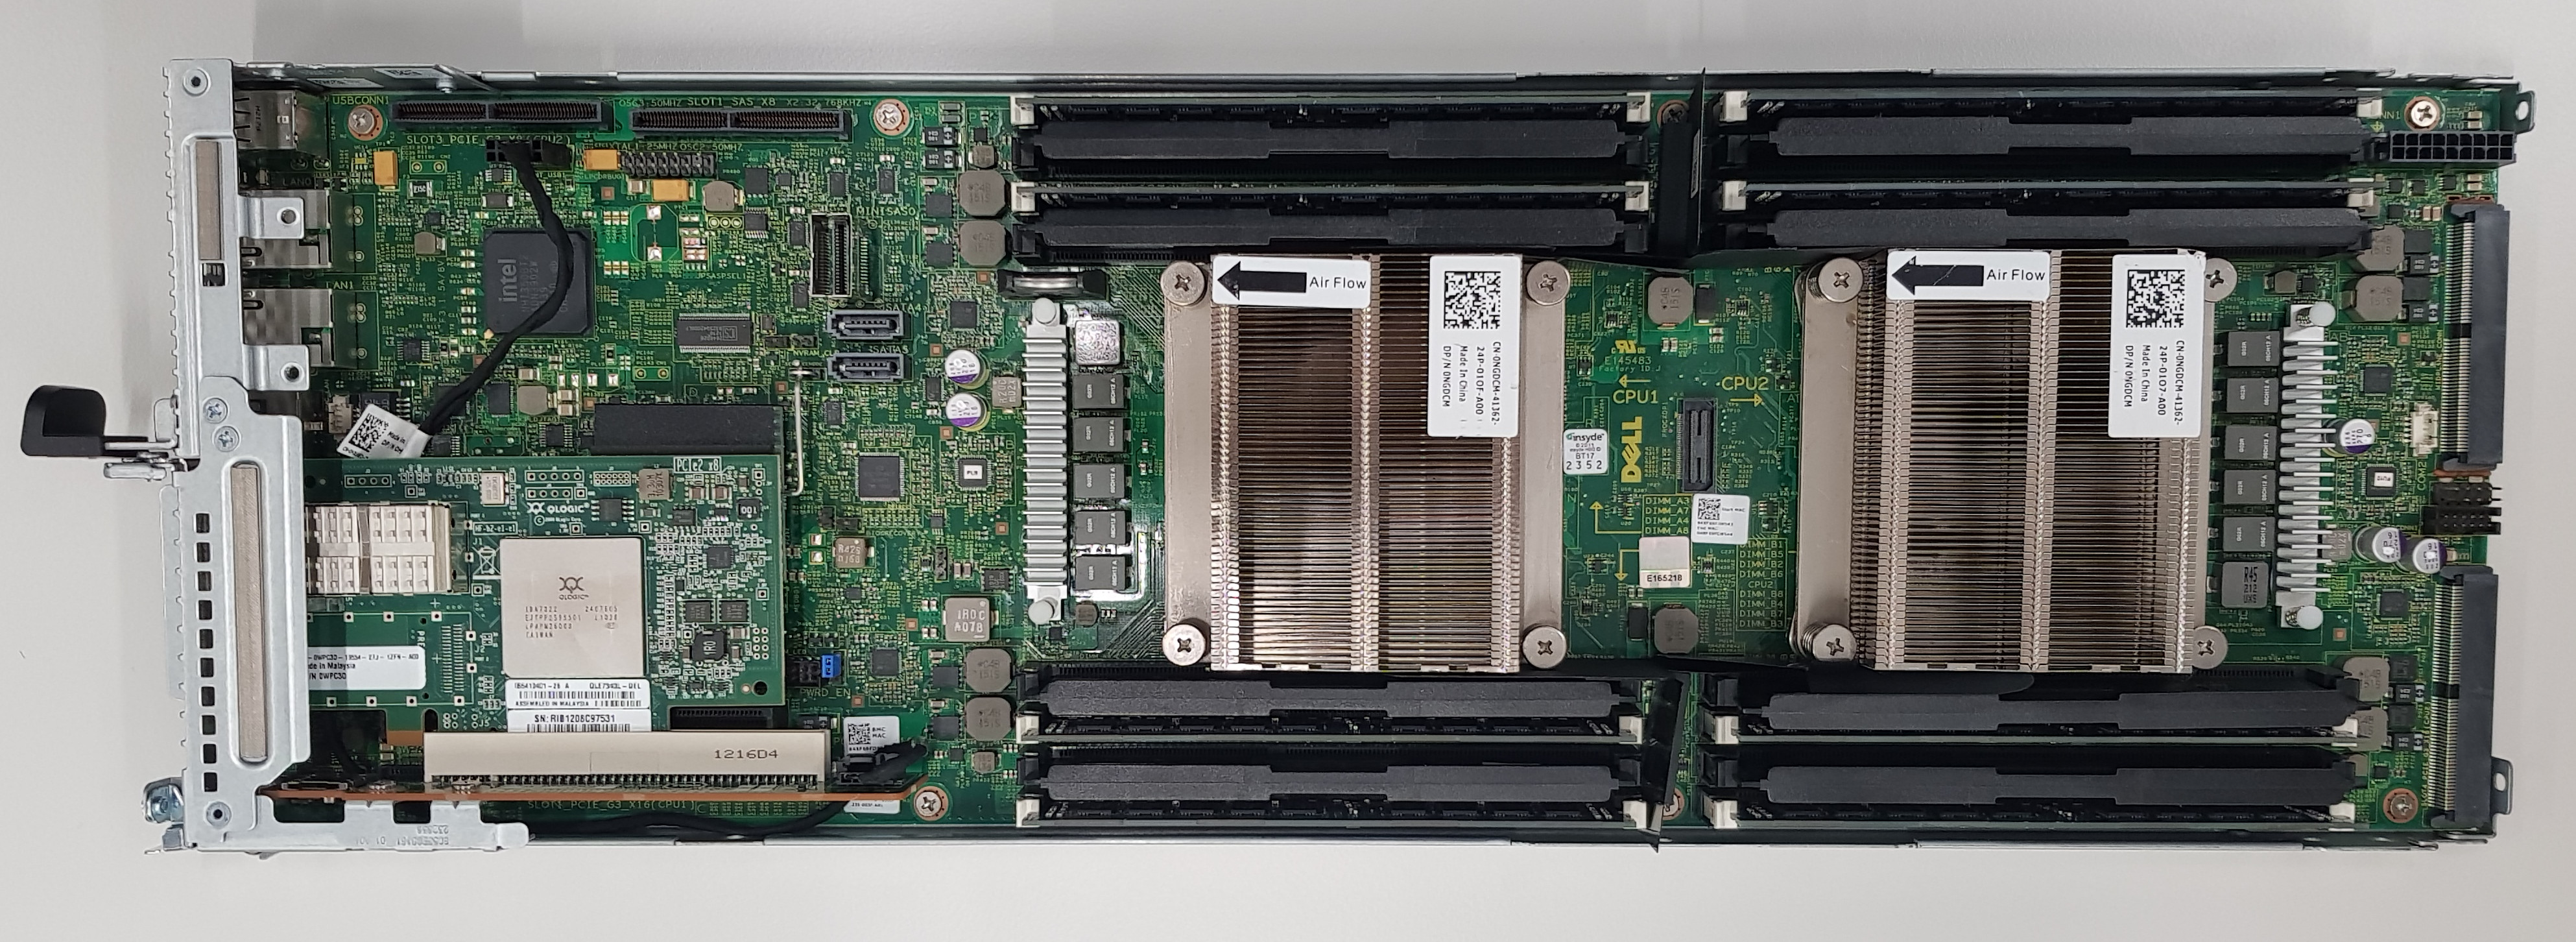
\includegraphics[height=4cm]{Day0/images/bellatrix-node.jpg}}
\end{center}
\end{frame}

\begin{frame}[containsverbatim]
\frametitle{Some important values}
\begin{itemize}
	\item{\textbf{CPU performance} measured in FLOPS (Floating Point Operations Per Second).}
	\item{\textbf{Memory bandwidth} in Bytes per second}
	\item{\textbf{Memory latency} in seconds}
\end{itemize}
It is usual to give the \textbf{peak} values (never reachable) defined by :
\begin{itemize}
	\item{\textbf{Peak CPU performance =} CPU Frequency \textbf{X} Number of Operations per clock cycle \textbf{X} size of the largest vector \textbf{X} number of cores }
	\item{\textbf{Memory bandwidth = } RAM Frequency \textbf{X} Number of transfers per clock cycle \textbf{X} Bus width \textbf{X} number of interfaces }
	\item{\textbf{Memory latency } depends on the size of the data. Usualy given by the constructor}
\end{itemize}
\end{frame}


\begin{frame}[containsverbatim]
\frametitle{Benchmarks to measure the values}
\begin{itemize}
	\item{\textbf{CPU performance} : HPL (LINPACK)}
	\item{\textbf{Memory bandwidth} : STREAM or PMBW }
	\item{\textbf{Memory latency} : Intel Memory Latency Checker}
\end{itemize}
\end{frame}

\begin{frame}[containsverbatim]
\frametitle{HPL (High Performance LINPACK)}
\begin{itemize}
	\item{Invented by Jack Dongarra (ORNL) in 1979}
	\item{solves a $n$ equations with $n$ unknown linear system $A x = b$ using Gauss partial pivoting}
	\item{This is the current benchmark for parallel computer. But it can be used to benchmark a single node or machine}
\end{itemize}
\end{frame}



\begin{frame}[containsverbatim]
\frametitle{HPL results}
\tiny
\begin{verbatim}
================================================================================
T/V                N    NB     P     Q               Time                 Gflops
--------------------------------------------------------------------------------
WR11C2R4       81792   192     4     4            1421.16              2.567e+02
HPL_pdgesv() start time Tue Oct 16 16:11:34 2018

HPL_pdgesv() end time   Tue Oct 16 16:35:15 2018

--VVV--VVV--VVV--VVV--VVV--VVV--VVV--VVV--VVV--VVV--VVV--VVV--VVV--VVV--VVV-
Max aggregated wall time rfact . . . :               6.67
+ Max aggregated wall time pfact . . :               4.28
+ Max aggregated wall time mxswp . . :               3.88
Max aggregated wall time update  . . :            1414.90
+ Max aggregated wall time laswp . . :             497.88
Max aggregated wall time up tr sv  . :               0.92
--------------------------------------------------------------------------------
||Ax-b||_oo/(eps*(||A||_oo*||x||_oo+||b||_oo)*N)=        0.0016200 ...... PASSED
================================================================================
\end{verbatim}
\end{frame}

\begin{frame}[containsverbatim]
\frametitle{HPL results on one Fidis node (f104)}
\tiny
\begin{verbatim}
================================================================================
T/V                N    NB     P     Q               Time                 Gflops
--------------------------------------------------------------------------------
WR11C2R4       81792   192     4     4             622.06              5.864e+02
HPL_pdgesv() start time Thu Oct 18 16:32:50 2018

HPL_pdgesv() end time   Thu Oct 18 16:43:12 2018

--VVV--VVV--VVV--VVV--VVV--VVV--VVV--VVV--VVV--VVV--VVV--VVV--VVV--VVV--VVV-
Max aggregated wall time rfact . . . :               2.51
+ Max aggregated wall time pfact . . :               0.64
+ Max aggregated wall time mxswp . . :               0.27
Max aggregated wall time update  . . :             619.19
+ Max aggregated wall time laswp . . :              27.47
Max aggregated wall time up tr sv  . :               0.24
--------------------------------------------------------------------------------
||Ax-b||_oo/(eps*(||A||_oo*||x||_oo+||b||_oo)*N)=        0.0017884 ...... PASSED
================================================================================
\end{verbatim}
\end{frame}



\begin{frame}[containsverbatim]
\frametitle{Memory bandwidth example}

\begin{center}
\includegraphics[page=61,width=.9\textwidth]{Day0/images/plots-scitaspc3-p1.png}
\end{center}

\end{frame}

\begin{frame}[containsverbatim]
\frametitle{Intel Memory Latency Checker (1/3)}
\tiny
\begin{verbatim}
Intel(R) Memory Latency Checker - v3.5
Measuring idle latencies (in ns)...
		Numa node
Numa node	     0	     1	
       0	  76.2	 122.9	
       1	 123.3	  75.7	

Measuring Peak Injection Memory Bandwidths for the system
Bandwidths are in MB/sec (1 MB/sec = 1,000,000 Bytes/sec)
Using all the threads from each core if Hyper-threading is enabled
Using traffic with the following read-write ratios
ALL Reads        :	101136.4	
3:1 Reads-Writes :	93459.2	
2:1 Reads-Writes :	93216.4	
1:1 Reads-Writes :	90454.1	
Stream-triad like:	81659.8	

Measuring Memory Bandwidths between nodes within system 
Bandwidths are in MB/sec (1 MB/sec = 1,000,000 Bytes/sec)
Using all the threads from each core if Hyper-threading is enabled
Using Read-only traffic type
		Numa node
Numa node	     0	     1	
       0	50481.0	 8451.7	
       1	 8415.8	50533.1	
\end{verbatim}
\end{frame}

\begin{frame}[containsverbatim]
\frametitle{Intel Memory Latency Checker (2/3}
\tiny
\begin{verbatim}
Measuring Loaded Latencies for the system
Using all the threads from each core if Hyper-threading is enabled
Using Read-only traffic type
Inject	Latency	Bandwidth
Delay	(ns)	MB/sec
==========================
 00000	170.22	 102119.1
 00002	172.92	 102090.6
 00008	176.54	 101964.0
 00015	199.00	 100029.4
 00050	174.13	  94163.3
 00100	135.42	  60156.9
 00200	119.19	  37658.6
 00300	132.01	  27635.2
 00400	122.57	  21903.4
 00500	100.41	  18037.9
 00700	 95.57	  13667.4
 01000	 93.79	   9701.4
 01300	 90.08	   7806.2
 01700	 94.09	   6234.9
 02500	 90.04	   4575.8
 03500	 85.77	   3515.6
 05000	 88.68	   2670.1
 09000	 86.89	   1830.2
 20000	 90.07	   1203.9
\end{verbatim}
\end{frame}


\begin{frame}[containsverbatim]
\frametitle{Intel Memory Latency Checker (3/3}
\tiny
\begin{verbatim}
Measuring cache-to-cache transfer latency (in ns)...
Local Socket L2->L2 HIT  latency	30.8
Local Socket L2->L2 HITM latency	35.5
Remote Socket L2->L2 HITM latency (data address homed in writer socket)
			Reader Numa Node
Writer Numa Node     0	     1	
            0	     -	  86.4	
            1	  86.3	     -	
Remote Socket L2->L2 HITM latency (data address homed in reader socket)
			Reader Numa Node
Writer Numa Node     0	     1	
            0	     -	  86.1	
            1	  86.4	     -	
\end{verbatim}
\end{frame}




\begin{frame}[containsverbatim]
\frametitle{Roofline model}
\begin{center}
        {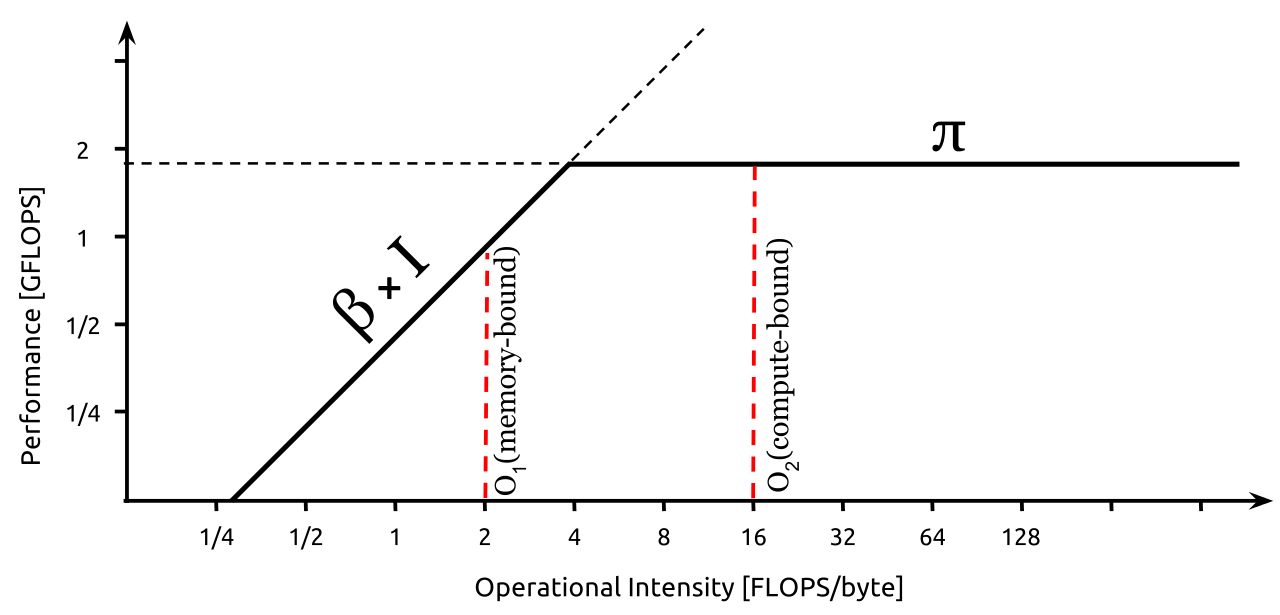
\includegraphics[height=5cm]{Day0/images/roofline.png}}
\end{center}
\end{frame}



